\chapter{Introduction}

\section{Overview of Distributed Sensor Networks}
Distributed sensor networks (DSNs) consist of any number of sensors that collect and sense information about the physical environment around them. The sensors that make up these networks can either be homogeneous or heterogeneous. Distributed sensor networks are dynamic in that sensors can be added or removed from the network at any time. DSNs also increasingly include mobile sensors as well. With the onset of the Internet of Things (IoT), its easier than ever to build and deploy distributed sensor networks. Further, mobile devices, such as mobile phones, are seeing increased usage as intelligent sensing agents.

\subsection{DSN Data Collection Schemes}
Data can be collected from DSNs in various ways. Sensors can store data onboard to be collected manually or transmit data via a multitude of mediums (satellites, radio, laser, wired connections) using a slew of standards (TCP/IP, Zigbee, Bluetooth, custom, etc).

In some DSNs, data is routed between the sensors using various approaches and eventually makes its way to a sink or sinks. A sink is a data collection node. Cloud computing has become a prevalent choice for DSN sinks since they often provide the ability to provision resources as needed. Various approaches have been proposed that minimize and optimize communications between sensors within a DSN.

In other DSNs, sensor nodes have direct access to a sink, and instead of communicating with each other and passing messages among themselves, the nodes send their data directly to the sink. It's also possible for a DSN to take a hybrid approach and performs some communication within the network and some directly to the sink.

Not only are there various approaches to routing data, but there are also various approaches to deciding what kind of data to send (or acquire).

\subsection{DSN Detection Schemes}
On one extreme end, we have the send everything approach where each sensor sends its data to the sink all the time (or at least when it has the means to do). In this scenario, the sink is responsible for collection, cleaning, detection, and classification of signals and events within the data. This approach can be bandwidth and energy intensive, but provides the benefit of allowing more complete analysis to occur beyond the sink where more computational resources exist. This provides more accurate results and allows the sink to examine the results in aggregate with the rest of the DSN.

The other extreme is that sensors only send data when they have detected a signal of interest. In this scenario, sensors use onboard computing capabilities to filter their sensor stream and perform signal detection on the device. Only when the devices make a detection do they send the detection or data stream to a sink for further processing. This minimizes bandwidth but detection and classification of signals must occur with more constrained computing and energy environments. Further, the global state of the network can't be known without adding the complexity of sensor-to-sensor communication.

Often time a hybrid approach is taken where low fidelity feature extracted and sometimes aggregate data is sent from the sensors to the sink. The sink analyzes the low fidelity feature extracted stream to determine if raw data should be requested from the sensors. The act of requesting data from the sensors is called triggering. This approach is useful because we still gain bandwidth benefits and can easily gain an understanding of the global state of a network.

With all of these factors combined, management, collection, detection, localization, and analysis from distributed sensor networks is not a trivial task. DSNs can produce massive amounts of data. The emergence of IoT has increased the heterogeneity of sensors with multiple hardware configurations, variations of data APIs, and incomplete or bad sensor data. For these reasons, the data collected from distributed sensor networks under certain circumstances is considered Big Data.

\subsection{DSN Classification Schemes}
% TODO

\subsection{DSNs as Big Data}
Big Data is generally defined by the four V's; volume, velocity, variety, and value. These characteristics can be observed in many of the DSNs that exist and are being created today. % TODO more citations

That is, distributed sensor networks create a large volume of data due to the abundance of IoT and mobile devices that make up DSNs. As communication infrastructures improve and hardware becomes smaller, smarter and more energy efficient, sensors are able to send and transfer larger amounts of data. The ease of building and deploying sensors in DSNs means that more sensors can be produced much more cheaply allowing for more sensors to be used within a DSN, increasing coverage, but also increasing the volume of data.

Distributed sensor networks create a variety of data with different formats and data quality issues. Distributed sensor networks can produce data at high velocity. These characteristics of data produced from distributed sensor networks create a need for efficient architectures and specific algorithms designed for working with Big Data.

Further, sensor networks are often constrained in both computing power and available energy sources. This forces us to find comprises between data collection, onboard sensor processing, sensor communication, and network coordination.

\section{The Data Management and Analysis Problems}
All DSNs must decide how data is managed and analyzed. There are various approaches 

\section{Traditional Approaches to Data Management and Analysis}

\section{Seven proposed benefits of Laha} \label{laha-benefits}
Laha is designed to adaptively optimize the collection, triggering, detection, and classification of signals within a DSN. These optimizations provide several benefits to DSNs.

\subsection{Tiered management of Big Data}
% TODO If you're going to use "Big Data" as a term of art, then it needs to be rigorously defined.
% TODO What I think you need to emphasize here is that in any Big Data scenario, you simply can't keep all the data around forever. So, what approach will be used to decide what data to keep and what data to discard?  Laha addresses this problem by having a series of levels, each with its own TTL.  This approach has the benefit of simplifying the analysis of bandwidth and storage requirements for a DSN, but at the cost of potentially discarding important data due to the "use it or lose it" design.  Part of youer evaluation should attempt to address this weakness of use it or lose it.

Laha provides tiered management of the Big Data that the framework consumes. This is mainly accomplished using the layered approach that Laha provides. All data within the Laha framework is garbage collected using a configurable time to live (TTL) for each layer. As data moves from the bottom to the top of the framework, noise is discarded and only interesting data as determined by the higher layers is preserved and forwarded upwards within the framework. In this way, the network can be tuned to preserve increasingly important data. The details of Laha's tiered approach can be found in section \ref{big-data-management}.

\subsection{Automatically provide context to classified incidents}
% TODO This is a feature that will be hopefully much more easily evaluated once you have the two reference implementations.  I will be interested to see what kinds of contextual information are attached, and whether there are times you wished you could attach information elsewhere.
Laha provides Annotations Phenomena (see \ref{annotations-phenomena}) that allows users or algorithms to tag signals of interest with contextual information. There is already a large amount of research for providing classifications of signals of interest, however annotations provide context about the classifications themselves. That is, Laha provides the ability to assign causality to already classified signals.

Initially, a library of annotations is required to be built for a particular DSN. Once the library has been built, Laha can provide automatic annotation assignment using similarity metrics. By using annotations and determining causality, it's possible to create actionable responses to signals observed within a network.

Further, annotations can be used to optimize detection and classification of known signals. For example, imagine a power quality network that observes a voltage sag on the same sensors at the same time periodically. If the cause of the voltage sag can be determined (such as a motor turning on), then detection of this signal can either be muted or analyzed more deeply. Also, other voltage sags that exhibit similar characteristics can then be automatically annotated.

\subsection{Adaptive optimizations for triggering}
% TODO This seems totally cool, but I question whether this is a novel feature. Adaptive setting of thresholds must happen in lots of different domains.  You'll want to discuss related work here, and hopefully argue that other approaches are ad-hoc and domain-specific, but the contribution of Laha is to build adaptive optimization of triggering directly into the framework as a first-class concept. 
Many triggering schemes rely on thresholds being surpassed within feature extracted data streams. For example, triggered data streams in a power quality network might consist of voltage, frequency, and THD extracted features to determine if there is likely a signal of interest observed from a given set of sensors. If any of the extracted features surpass a preset threshold, then we  end up triggering the devices for raw, higher fidelity data. However, there are cases where the feature extracted stream may not surpass a predefined threshold and those sensors would not be triggered.

By using different types of Phenomena, we can improve our triggering efficiency. For example, Locality Phenomena, as discussed in section \ref{locality-phenomena}, allow us to predict detections and classifications in space. If a particular grouping of sensors that are related in space always observe the same detections and classifications, then we can build a predictive model of when the framework can expect to see those things. In this way, a sensor may trigger on a passed threshold, but other sensors that are co-located may not trigger because feature extracted data is below the triggering threshold. If the Locality Phenomena predicts that other co-located sensors should have detected the same signal, then we might trigger those devices for high fidelity data to determine if the signal is in the raw data stream even though it didn't meet the triggering threshold.

Laha can use Periodicity Phenomena, as discussed in section \ref{periodicity-phenomena}, in similar ways. When periodic signals are classified, we can create Future Phenomena that predicts when signals of interest should be detected and classified. This allows Laha to optimize triggering by tuning the triggers to specifically look for Periodic or Future Phenomena. Periodic and Future Phenomena also allows Laha to tune classification algorithms to the predicted classifications.

\subsection{Adaptive optimizations for detection and classification}
Not only can Laha optimize triggering, but similar usages of Locality and Future phenomena can be utilized to improve detection and classification efficiency. With Locality Phenomena, a model of common detections and classifications can be built for a set of co-located sensors. Detection and classification algorithms can be tuned to search for specific signals that are often observed within this model, pruning the search space and increasing the accuracy of detection and classification algorithms.

Future and Periodic Phenomena provide the same benefits to detection and classification as Locality Phenomena. That is, if Laha is able to predict when a signal is going to arrive and also predict how that signal is going to be classified, then it can tune its detection and classification algorithms specifically for the signal of interest.

\subsection{Provides a model of underlying sensor field topology}
% TODO Either this is extremely cool, or totally frivolous, and I'm not sure which. it is frivolous if the only thing it's doing is detecting topology that you already know about (i.e. that two OPQ boxes are close together physically, but we already know that because of their lat/long coordinates.) it is totally cool if you are detecting topology that is not already known. So, it would be good to provide a specific example here for both domains (OPQ and Lokahi)

Predictive phenomena use localization of signals to build communities or groupings of sensors that observe similar signals in both time and space. Over time, Laha can begin to build a model of the underlying topology of the sensing field. For instance, if a group of sensors always see the same signal, then we can assume that either the signal has a far reach, or the sensors are grouped together geographically. With enough sensor penetration, we can differentiate between these two scenarios.

Further, if the sensors provide any sort of location information, Laha can provide a mapping from physical location to sensor field topology. This is especially useful when the topology of the sensor field is not known a priori. Even if we know the location of the sensors at all times, that does not mean that we understand the topology of the sensing field. For example, in a PQ network, the topology is defined by how the electrical grid is connected to itself and laid out. Laha hopes to provide a model that can determine the electrical distance between devices even if the topology of the grid is not known. As another example, take an infrasound network. It's possible that two sensors are located close to each other geographically, but if they have a large mass between them, they may not receive the same signals due to the topology of the environment around them. 

In this sense, Laha is not interested in knowing the location of sensors relative to each other, but is more interested in understanding how signals flow between sensors as a constraint on the topology that the signals travel through.


\subsection{Decreased bandwidth of entire DSN}
One of the tertiary benefits of optimizing triggering and classification is that we get decreased bandwidth usage for free. By improving triggering efficiency, its possible to trigger less devices for raw data when something interesting is observed in the triggering stream.

Predictive phenomena allow us to target triggers to sensors that are most likely to have captured a signal of interest. For instance, if a geographical grouping of sensors tend to always observe the same signals of interest, then we can use that grouping to optimize triggering. Instead of triggering all devices in an area to search for the signal, we can trigger only on the specific grouping that is most likely have observed the signal. We can also selectively ignore sensors within a predictive grouping if Laha assumes that all sensors observed the signal, then we may only need to analyze the signal from one of the sensors rather than all of the sensors in the grouping.

\subsection{Minimizing sensor power requirements}
In general, sensors are both compute and energy constrained. Most of the time, communications are the main source of sensor device power requirements within a DSN.

In an energy constrained DSN where communications amount for the most usage of energy, decreased bandwidth also provides decreased sensor device power requirements. This can prolong the life of DSNs or provide more energy for other parts of the network (such a pushing computations to the edge).

\section{Evaluation of Laha}
\subsection{Design and implement Laha-compliant software reference implementations (OPQMauka and Lokahi)}
OPQMauka is a distributed, plugin-based middleware component of the Open Power Quality (OPQ) software stack that provides higher level analytics and data management for a distributed PQ network.

\subsubsection{Open Power Quality}
OPQMauka is a middleware component of the Open Power Quality (OPQ) framework. The OPQ project provides a hardware and software solution for monitoring distributed power quality (PQ). The OPQ project was founded with the goal of studying how intermittent distributed renewable energy sources affect PQ not just at a user's home, but also within a user's neighborhood, between neighborhoods, and globally across the grid. 

The OPQ ecosystem is made up of networked hardware sensors (OPQBoxes) and various software services (OPQMakai, OPQMauka OPQHealth, OPQView). Each of these software components are made up of individual services and plugins.

The OPQ system design is laid out in figure \ref{fig:opq-system}.

\begin{figure}
	\centering
	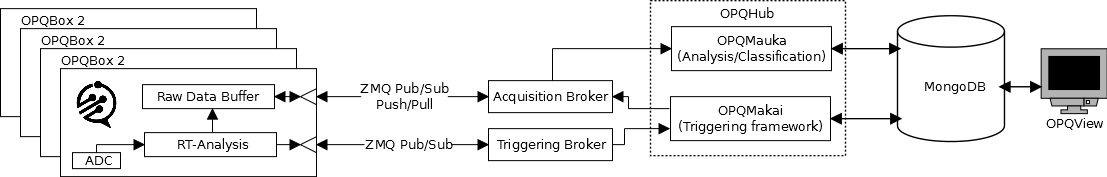
\includegraphics[width=\linewidth]{figures/system-diagram.png}
	\caption{OPQ System Diagram}\label{fig:opq-system}
\end{figure}

\subsubsection{OPQ: Boxes}
An OPQ Box is a custom designed PQ sensor. OPQBoxes can be plugged into a wall outlet and communicate with OPQ servers using the user's WiFi connection. OPQBoxes consist of a Raspberry PI single board computer (SBC), a custom board for PQ measurements, custom firmware, and a custom enclosure. The custom board contains an ADC that samples an alternating current (AC) power signal at 12 thousand samples per second. This data is transferred to the Raspberry Pi where feature extraction and data transfer takes place. The hardware design is presented in figure \ref{fig:opq-box-design} and the software design is provided in figure \ref{}.

\begin{figure}
	\centering
	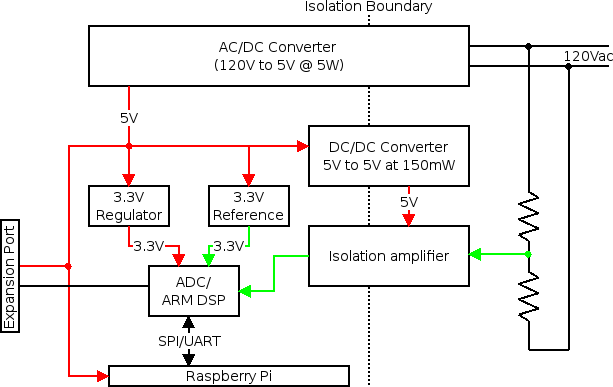
\includegraphics[width=.75\linewidth]{figures/opqbox_diagram.png}
	\caption{OPQ Box Design}\label{fig:opq-box-design}
\end{figure}

\begin{figure}
	\centering
	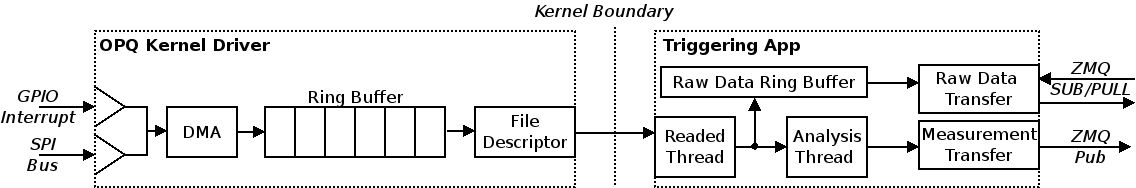
\includegraphics[width=.75\linewidth]{figures/opqbox_software.png}
	\caption{OPQ Box Software}\label{fig:opq-box-software}
\end{figure}

The feature extraction algorithms extract from the sampled waveform the following features: windowed $V_{RMS}$, frequency, and total harmonic distortion (THD) features. The feature extracted data is then sent to a central sink where further analysis is used to determine if the sensor or a subset of sensors should be triggered for raw data.

The OPQ network is a hybrid network that uses edge computing for calculating features at the edge of the network. This is opposed to networks that utilize a ``send everything" approach. In this way, we are able to minimize bandwidth. 

OPQBoxes are synchronized to each other and the OPQ back end using the network time protocol (NTP). This provides synchronization to the millisecond level, which although is great for longer incidents, does not provide accurate timing for transients that may be shorter than tens of milliseconds.


\subsubsection{OPQ: Makai}
OPQ Makai is the central sink and triggering daemon for the OPQ framework. It is made up of several services which are responsible for aggregating and processing the measurements generated by OPQ Boxes. Low fidelity feature extracted data consisting of $V_{RMS}$, frequency, and THD are streamed from OPQ Boxes at a configurable message rate. These data streams are observed by OPQ Makai and the daemon uses statistical methods and thresholds to determine if the sensor or a subset of sensors should be triggered for a window of raw sampled waveforms. 

The OPQMakai system design is provided in figure \ref{fig:makai-main}.

\begin{figure}
	\centering
	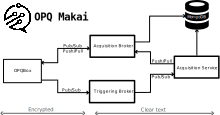
\includegraphics[width=.75\linewidth]{figures/makai_main.pdf}
	\caption{OPQ Makai Design}\label{fig:makai-main}
\end{figure}

\subsubsection{OPQ: Health}
OPQHealth is a service that continuously monitors both the hardware sensors and the software services that make up the OPQ framework.

OPQHealth detects health issues in the following ways. 

OPQHealth determines if an OPQBox is active or inactive by querying the Mongo database for the most recent aggregate measurement. If there is a record of an aggregate measurement within 5 minutes, the Box is considered up, otherwise it is considered down.

The status of OPQMakai is determined by Makai inserting special health events into the Mongo database. Health queries for the presence of these events and if events are not observed within 1 minute, the OPQMakai service is considered down.

OPQMauka provides a special HTTP endpoint that is only accessible within the OPQ back end network that when accessed with a \textit{GET} request will return with a status of \textit{200 OK} if the service is up and available. Any other response of the absence of the response is considered a failure more for OPQMauka.

MongoDB is monitored by querying for a sentinel value that was previously placed in the database.

OPQView is monitored by sending a \textit{GET} request to the landing page. A response of \textit{200 OK} means that the health service is up. Any other response or the lack of response is an indication of failure for OPQView.

OPQHealth stores its findings in both the Mongo database as well as in a traditional log file.

\subsubsection{OPQ: View}
OPQView is a web application that provides visualization, notification, and user management services for data, sensors, and user accounts with the OPQ framework. OPQView is built using Meteor.js and provides a Reactive view of the underlying data stored in the OPQ database.

A screenshot of OPQView in action is provided in figure \ref{fig:opq-view}.
	
\begin{figure}
	\centering
	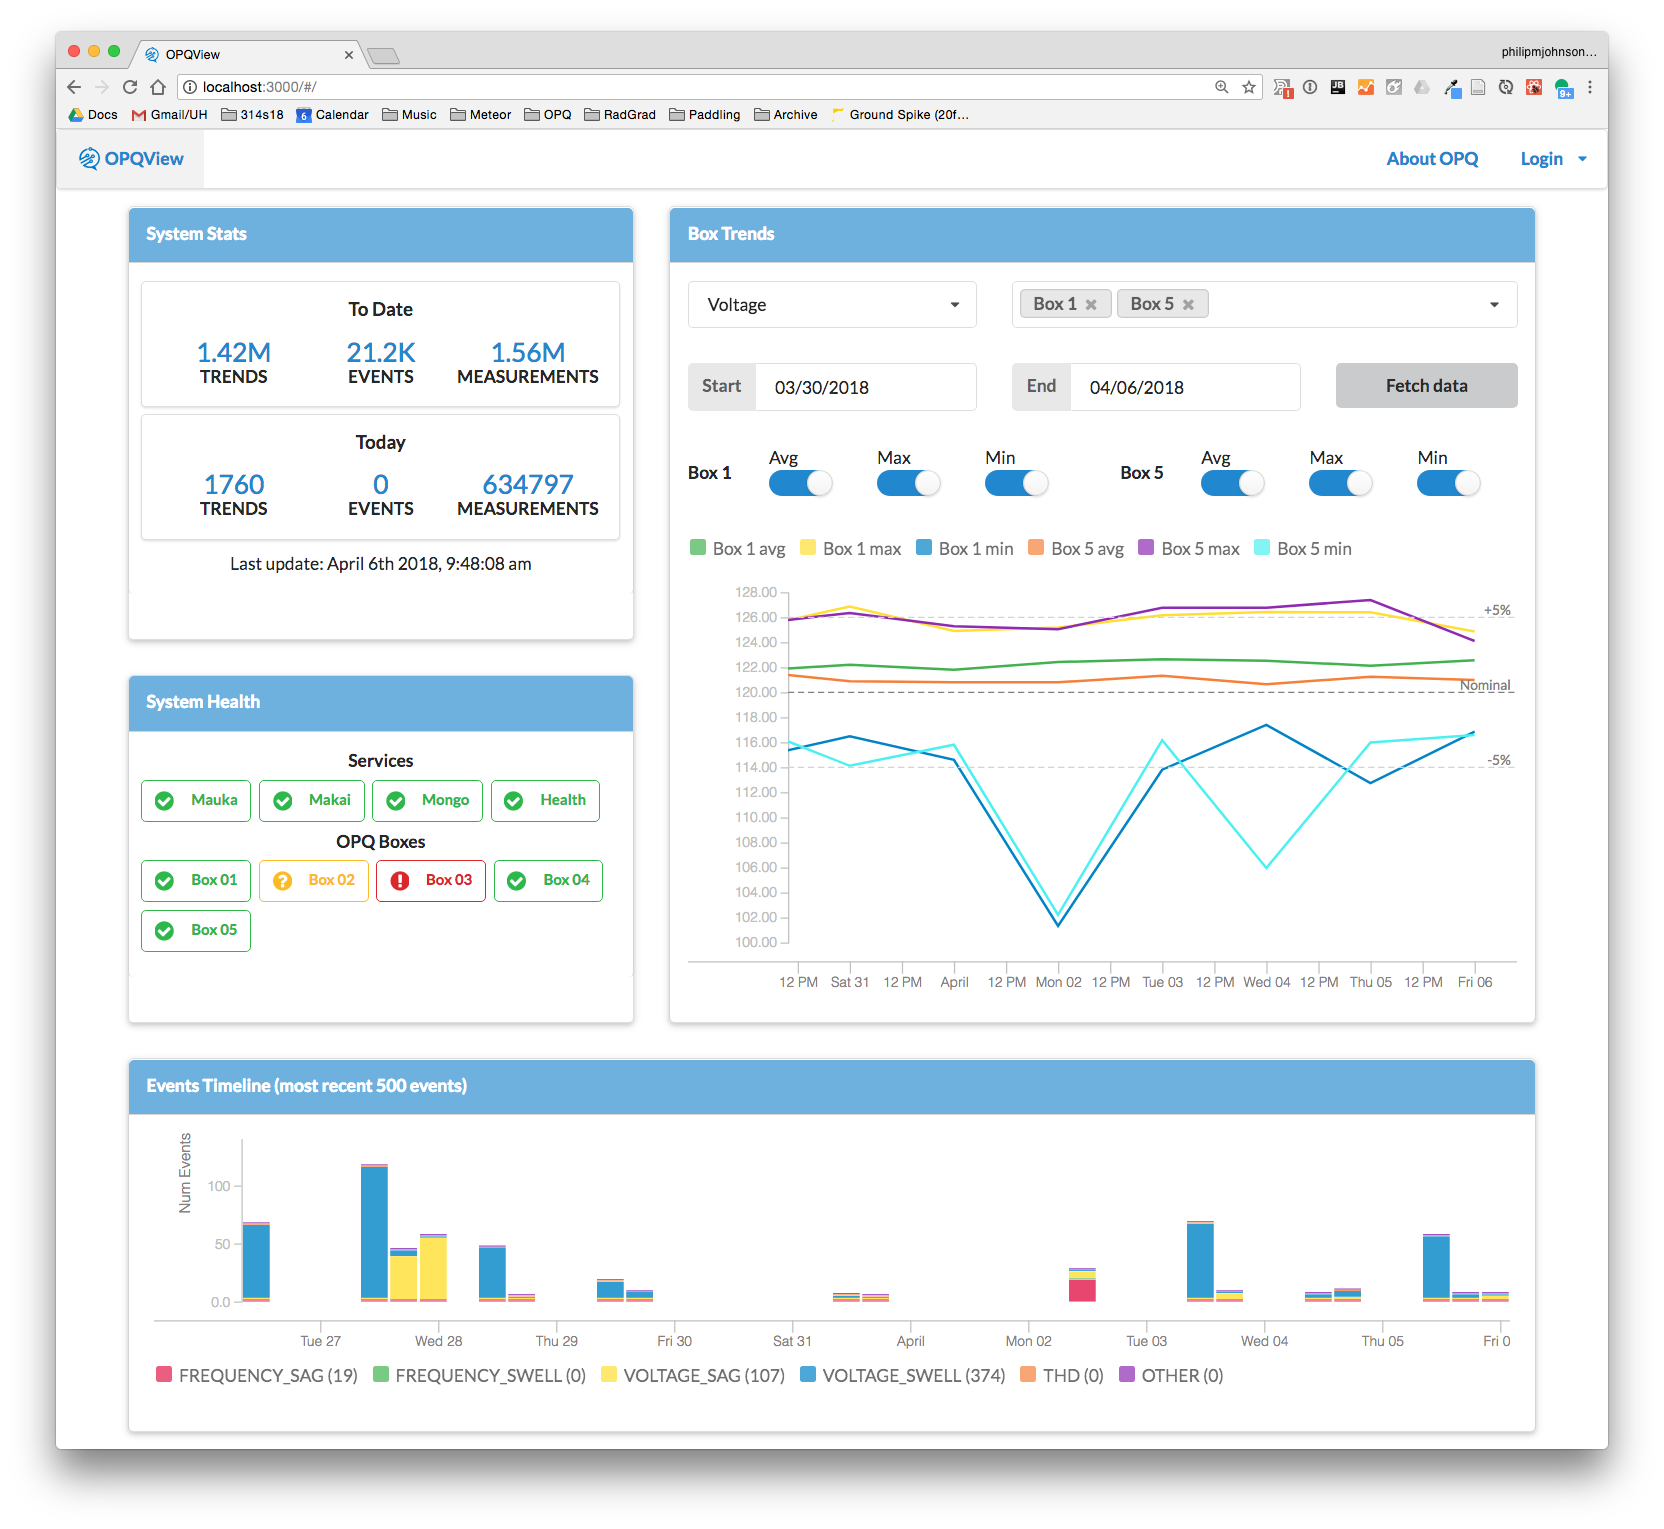
\includegraphics[width=1\linewidth]{figures/opqview-landing-page.png}
	\caption{OPQ View Screenshot}\label{fig:opq-view}
\end{figure}

\subsubsection{OPQ: Mauka}
% TODO

TODO: This section is in the making and will be much more detailed than the other components of OPQ.

\subsubsection{OPQ: Data Model}
% TODO

\subsubsection{OPQ as a Laha-compliant DSN}
OPQ and specifically OPQMauka comply with the Laha abstract framework. Table \ref{opq-compliance} summarizes how the OPQ data architecture fits within the Laha conceptual model.

\begin{table}
	\caption{OPQ as a Laha-compliant DSN}
	\begin{tabular}{|c|c|c|c|c|}
		\hline 
		Laha Layer & OPQ & Created By & Stored By & TTL \\ 
		\hline 
		IML & raw ADC Samples & OPQBox & Onboard memory & 20 minutes \\ 
		\hline 
		AML & min,max,avg V, F, THD & OPQBox & trends\footnotemark & 1 day \\ 
		\hline 	
		DL & triggered waveforms & Makai/Mauka & events/box\_events\textsuperscript{\ref{fn-1}} & 1 week \\
		\hline
		IL & Classified detections & Mauka & incidents\textsuperscript{\ref{fn-1}} & 1 year \\
		\hline
		PL & Predictive analytics & Mauka & phenomena\textsuperscript{\ref{fn-1}} & N/A \\
		\hline
	\end{tabular}
\label{opq-compliance}
\end{table}  
\footnotetext{MongoDB Collection Name\label{fn-1}}

In order to be a Laha compliant DSN, the reference DSN must also implement Laha Actors. Table \ref{opq-actors} summarizes how OPQ implements Laha actors.

\begin{table}
	\caption{OPQ  Actors Implementation}
	\begin{tabular}{|c|c|c|}
		\hline 
		Laha Actors & OPQ Equivalent & Description \\ 
		\hline
		IML Actors & Boxes & Store window of raw sensor samples \\
		\hline
		AML Actors & Boxes \& Makai & Makai stores and triggers on aggregate data from Boxes \\
		\hline
		DL Actors & Mauka & MakaiEvent plugin \\
		\hline
		IL Actors & Mauka & Voltage, Frequency, THD, Outage, plugins \\
		\hline
		PL Actors & Mauka & Annotations, Locality, Similarity,  Periodic, Predictive,  Future plugins\\
		\hline
	\end{tabular}
	\label{opq-actors}
\end{table}  

\subsubsection{Lokahi}
Lokahi is a dynamic DSN that originally evolved as a distributed infrasound detection network. Infrasound is characterized as sound waves that are less than 20 Hz. Infrasound generally can not be deciphered by the human ear, but it can be detected using microphone and barometric pressure sensors. Any large movements of the atmosphere can produce infrasound. The Lokahi network was designed to supplement the International Monitoring System (IMS) for the capture  of undeclared and declared nuclear explosions. Lokahi has been successfully used to capture signals from volcanoes, hurricanes, aircraft, meteors, and other large atmospheric events. 

Sensors in Lokahi are any mobile device that can run iOS or Android. We have sensors distributed world wide. The software stack for Lokahi consists of a distributed actor system for data acquisition, MongoDB for metadata persistence, Apache Kafka for data queues and interprocess communication, Python and related scientific libraries for analysis, and a distributed key-value store for long term storage or sensor data.

Recent development and improvements to the data API have allowed Lokahi to begin accepting data from any of the available onboard sensors on iOS and Android devices. Even though the main focus is still infrasound, having access to all of the available sensors provides the ability to sense other sensor fields and to perform interesting data fusion techniques. 

A diagram of the Lokahi framework is provided in figure \ref{fig:lokahi}.


\begin{figure}
	\centering
	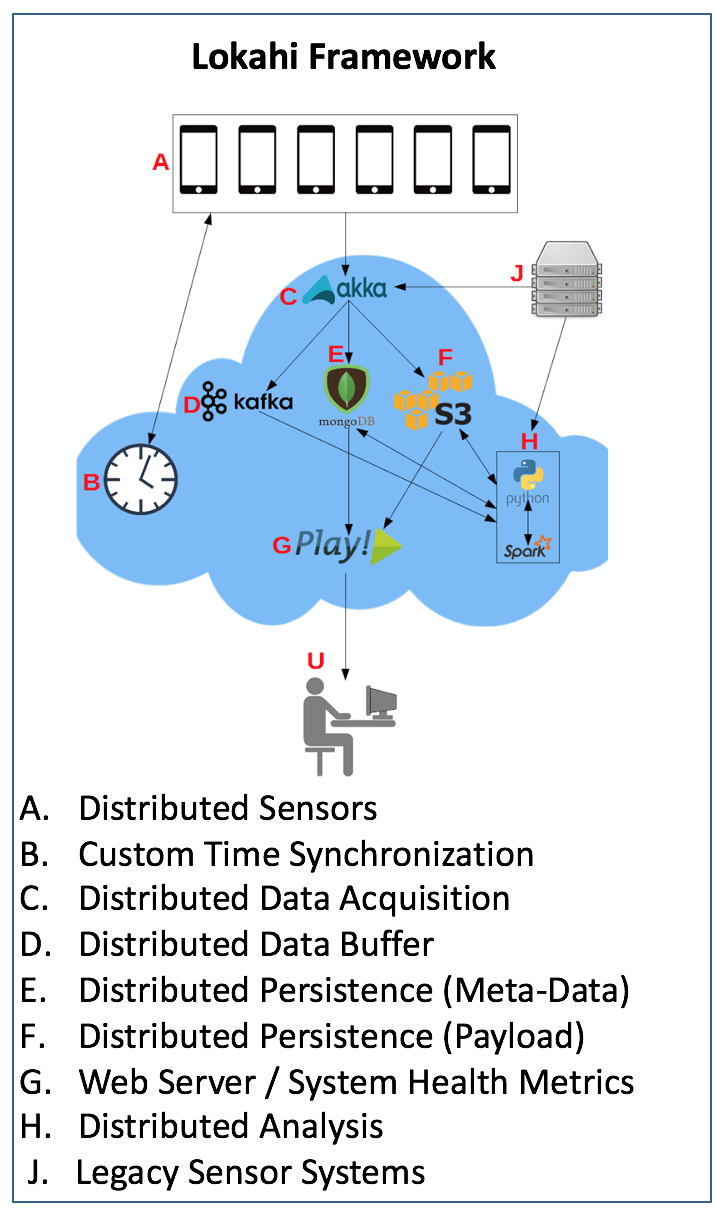
\includegraphics[width=\linewidth]{figures/lokahi.pdf}
	\caption{Lokahi Design}\label{fig:lokahi}
\end{figure}

\subsubsection{Lokahi: Ingestion}
Unlike OPQ, Lokahi takes an approach of send and store everything from every sensor, all the time. This approach is vastly different than what we're used to in triggering based acquisition systems. Data between sensors and our Ingestion servers is encrypted using standard SSL encryption algorithms. Authentication and authorization for each sensor is accomplished using Json Web Tokens (JWTs) with signatures generated using elliptic curve cryptography (ECC). Data at the sensor level is serialized using protocol buffers and then compressed using LZ4. 

To enable the smooth retrieval of large amounts of sensor data, Lokahi uses a distributed actor system (Akka) to automatically scale horizontally based on the current volume of data being received. 

\subsubsection{Lokahi: Persistence}
Metadata is stripped from the sensor data at data ingestion and immediate stored to a distributed Mongo database. Metadata is indexed using a combination of device id and timestamps. 

Metadata drives the rest of the Lokahi framework and provides pointers to the raw data.

Raw sensor data is stored in a distributed key-value store. Lokahi uses Amazon's Simple Storage Service (S3) which provides automatic data redundancy and essentially limitless storage. Raw sensor data is stored by key and the key is stored in the metadata.

Raw sensor data is also persisted in an Apache Kafka queue. Kafka not only provides the framework with a message queue to pass data between distributed services, but it also acts as a ring buffer. Each sensor stores 1 hours worth of data in Kafka that can be looked up by any of the distributed clients and retrieved very quickly. For those reasons, Kafka powers IPC and data buffering roles for our real time analysis of Lokahi sensor data streams.  

\subsubsection{Lokahi: Analysis}
Analysis in Lokahi is provided by a set of distributed processes that were developed in Python using SciPy, NumPy, and matplotlib. Recent developments in the framework are now also including the basis for machine learning (ML) using Tensor Flow.

We provide real time plotting and analysis by subscribing to real time data feeds provided by the Apache Kafka real time queue and buffer. We also provide more robust batch analysis of historical data that can be initiated from Lokahi Web.


\subsubsection{Lokahi: Web}
Lokahi web is a web application for querying and performing analysis of real time sensor data or over historical sensor data. Lokahi also has built in system of health displays for providing a real-time and historic overview of the health of the distributed services within the framework. 

% TODO, provide screenshot

\subsubsection{Lokahi as a Laha-compliant DSN}
%TODO

\subsection{Deploy Laha reference implementations on test sites}
In Q4 2018, 10 to 20 Laha-compliant OPQBoxes will be deployed on the University of Hawaii at Manoa's power microgrid. Using a provided blueprint of the microgrid as a guide and collaborating with the Office of Energy Management, these sensors will be placed strategically with the hopes of observing PQ signals on the same line, PQ signals generated from intermittent renewables, local PQ signals, global PQ signals, and PQ signals near sensitive lab electronics. Many of these sensors will be co-located with industry standard PQ monitoring systems. The industry standard sensors provide both ground truth and a means of comparison between a Laha powered network and a normal DSN. 

In Q4 2018,  20 to 30 Laha-compliant Lokahi sensors will be deployed near and around the Infrasound Laboratory in Kailua-Kona on the Big Island of Hawaii. These sensors will be placed strategically around a calibrated infrasound source. The sensors will be placed with the assistance of Dr. Milton Garces to ensure that we can target sensors at different distances by tuning the amplitude and frequencies of the infrasound signal. In this way, we know which devices should or should not have received the signal.

\subsection{Validate data collected by Laha deployment}
Beginning in Q1 2019, I will begin validated data collection from both the OPQ network and the Lokahi network. 

Data will be validated in the OPQ network be comparing detection and classified signals against industry standard meters that are co-located with our sensors. Data validation will be an autonomous process that validates signals seen in both the industry sensor and the OPQ sensor and also provides a means of quantifying the amount of signals that our sensors were not able to detect. 

Data from the Lokahi network will be validated against industry standard infrasound sensors. We also control the amplitude and frequency of the signals generated from the calibrated infrasound source and can use geophysical equations to predict which sensors should have seen or not seen an infrasonic signal. Data validation is autonomous for this network.

Data validation for both networks will continue for all data collection until the end of the project.

\subsection{Use Laha deployments to evaluate each of the seven proposed benefits discussed in section \ref{laha-benefits}}
The Laha deployments for both OPQ and Lokahi will be used to evaluate each of the proposed benefits discussed in section \ref{laha-benefits}. Each deployment offers different techniques for performing evaluation. 

In the OPQ deployment, OPQBoxes are deployed and co-located with industry standard, calibrated, reference sensors. Each of these sensors cost thousands to obtain and install, collect all the data all the time, and can only be connected to the power main as it enters a building. [TODO discuss the actual hardware and characteristics of the sensors installed by the office of power management at uh here]. These sensors provide a means for verifying signals received or not received by OPQ, as well as confirming long term trend data. I have been provided access to these sensors and stored data via the Office of Energy Management at UH Manoa. The data is accessible via an HTTP API. The Office of Energy Management at UH Manoa has also provided the full schematics for the UH power grid. This will be used as a ground truth for topology estimates and distributed signal analysis. OPQBoxes are placed in strategic locations on the UH Manoa campus specifically in order to evaluate the distributed nature of PQ signals. For example, OPQBoxes are placed on the same electrical lines as well as separate electrical lines to observe how PQ signals travel through an electrical grid.
% TODO discuss the actual hardware and characteristics of the sensors installed by the office of power management at uh here

In the Lokahi deployment, we have the opportunity to generate infrasound signals using a calibrated infrasound source. The source can be tuned to produce infrasound at configurable frequencies and amplitudes. The source works by attaching a variable pitch propeller to an electric motor that can be driven by a waveform generator. The source can generate signals that can be observed at large stand off distances, over tens of kilometers. Similar to the OPQ deployment, sensors within the Lokahi deployment will be co-located with industry standard, calibrated, infrasound sensors. These sensors can provide a metric of signals that were correctly observed, incorrectly observed, or not observed at all by the Lokahi deployment. [TODO characterize and provide details on these sensors] Further, infrasound itself is characterized quite well by various geophysical equations. These equations can be used to predict if sensors deployed in the Lokahi deployment are likely to observe generated infrasound signals.
% TODO discuss the actual hardware and characteristics of the sensors installed by the office of power management at uh here

\subsubsection{Evaluation of Tiered Management of Big Data}
During the acquisition and curating of data, metrics will be collected and stored about how much data is saved versus how much data is discarded at each layer within the Laha data hierarchy. These numbers will be compared against data storage as if the OPQ and Lokahi frameworks were to take a ``store everything" approach. Evaluation metrics provided will include percentage of data storage saved per data hierarchy layer as well as an estimate of overall decrease in data storage requirements for the entire DSN. 

I will also provide metrics on ``continuous storage pressure" which is a measure of the average amount of storage required at each layer given the current state of the network. That is, since data at all lower levels of the framework assigns a TTL to the data within the collection, the collection will exhibit a constant data pressure during sensor data collection. For example, at the lowest level, the IML collects raw data from all sensors all the time. Given the sample rate per sensor, the size per sample, the number of sensors, and a known TTL for this layer, we can estimate the maximum bounds of data management requirements that the IML requires. We can play similar estimation games with higher layers of the framework.

By removing data, Laha runs the risk of discarding data that contains signals of interest that our system was not able to detect or classify. 

By controlling the signals generated within the Lokahi DSN deployment, we can provide a measure of signals that were thrown out and not detected by our framework that would have been preserved if our framework took the approach of ``collect everything all the time". Similarly, calibrated reference sensors co-located with the OPQ deployment can provide metrics on signals that were observed by the reference sensors and subsequently thrown away and not observed within OPQ.

\subsubsection{Evaluation of Contextualizing Classified Incidents}
% TODO
[TODO: This is probably my weakest evaluation strategy of the 7 and I will continue to fill this one out this week].

To evaluate contextualized events, we will provide known. cyclical signals for both Laha deployments. We will first provide context for signals in both deployments as training data for the DSNs. Then, at difference distances from the source, I will reproduce the signals and will then provide a statistical error analysis for whether or not Laha is able to correctly contextualize the signals.

\subsubsection{Evaluation of Adaptive Optimizations for Triggering}
In order to evaluate triggering efficiency within our Laha deployments, Laha will only adaptively modify triggering for half of the devices the OPQ deployment. In the Lokahi deployment, we will run the same experiment twice. The first run will not optimize triggering and the second run will optimize triggering. Then, the following metrics will be tabulated to provide an evaluation for triggering efficiency:

\begin{itemize}
	\item Number of triggers performed from optimized devices versus number of triggers from  unoptimized devices
	\item Bandwidth requirements from optimized triggering versus bandwidth requirements from unoptimized triggering
	\item Storage requirements as a result of event storage from optimized triggering versus storage requirements from unoptimized triggering
	\item Detection, classification, and incident counts for optimized triggering versus detection, classification, and incident counts for unoptimized triggering
\end{itemize}

\subsubsection{Evaluation of Adaptive Optimizations for Detection and Classifications}
Evaluation of adaptive optimizations for detection and classification within the Laha network will be conducted differently for each Laha deployment.

In the Lokahi deployment, I will control the production of infrasound signals using the available infrasound source. I will run two experiments, where the amplitudes and frequencies of the signals are the same and the locations of the devices remain invariant. In the first experiment, Laha will not use optimized detection or classification provided by Phenomena. In the second experiment, Laha will use optimized detection and classification techniques provided by Phenomena. 

With known frequencies and amplitudes of the infrasound signals, we can compare the rate of detections and classifications between the optimized and unoptimized experimental runs. I expect to see a greater number of and more accurate detections and classifications from the optimized experiment.

In the OPQ deployment, we will compare the same metrics as the Lokahi deployment, but instead of controlling the source signal, we will co-locate OPQBoxes. In each pair of co-located OPQBoxes, one will be analyzed using Phenomena optimized detection and classification algorithms and the other will be analyzed using unoptimized detection and classification algorithms.

\subsubsection{Evaluation of Model of Underlying Sensor Field Topology}
To evaluate the model of the sensing field topology, I will take two different approaches for each Laha deployment.

In the Lokahi deployment, sensors will be strategically placed at different distances from the infrasound source. Some sensors will be close to each other geographically, but separated by terrain that infrasound signals will not easily travel through. By moving the infrasound source, we can expect to see infrasound signals arriving or not arriving at the sensors depending on the source and direction of the signal along with the physical features of the land. By performing multiple experiments, I hope to provide a model of the physical environment topology that Laha has built. I will compare Laha's model to the known topology and provide a statistical error analysis. 

In the OPQ deployment, sensors will be strategically placed on like and unlike electrical lines to observe how distributed PQ signals move through a power grid. In this deployment, Laha will build a topology model that doesn't show physical geographic distance between sensors, but instead will build a model of the electrical distance between sensors. This data will be evaluated by comparing the electrical distances found by the Laha model to the actual UH power grid as referenced by the schematic provided by the Office of Energy Management at UH Manoa. A statistical error analysis of the differences between electrical distances between the model and the schematic will be provided as an evaluation metric.

\subsubsection{Evaluation of Decreased Bandwidth of Entire DSN}
Bandwidth of the entire DSN can be evaluated by counting the number of bytes sent and received by the sink nodes in both Laha deployments. 

In the Lokahi deployment, I will run two separate experiments. The first without any Phenomena optimizations, and the second with all Phenomena optimizations. All other conditions (amplitude, frequencies, sensor locations) will remain invariant between experimental runs. We will then compare the total bandwidth used between experimental runs.

For the OPQ deployment, I will co-locate sensors with Phenomena optimizations applied for one of the two and Phenomena optimizations not applied to the other of the two. I will then compare total bandwidth usage between sensors that had optimizations versus those that did not utilize optimizations.

\subsubsection{Evaluation of Decreased Sensor Device Power Requirements of Entire DSN}
Sensor device power requirements will be evaluated separately for both OPQ and Lokahi deployments. 

In the Lokahi network, all sensors run off battery power. I will perform two experiments. In the first experiment all Phenomena optimizations will be disabled. In the second experiment, I will enable all Phenomena optimizations. We will start each experiment with full battery power for each sensor and we will record the rate of battery drain as well as the final battery usage at the end of each experiment. The experiments will be exactly the same in terms of signals produced and sensor configurations. The only difference will be whether or not all Laha optimizations will be enabled or disabled. 

In the OPQ deployment, we will attach a power consumption meter to a pair of co-located sensors. One sensor will use Laha optimizations, the other will now. I will measure and compare power consumption between the two sensors. 

\section{Anticipated contributions of this thesis}
\subsection{Laha design: a novel distributed sensor network adaptive design with seven useful properties}
\subsection{Laha evaluation: empirical data to confirm or deny the seven useful properties}
\subsection{OPQMauka and Lokahi: reference implementations of Laha}
\subsection{Implications for modern distributed sensor networks}

\section{Timeline}
\subsection{2018 Q4: Implement, deploy, and validate Laha reference implementations}
\subsection{2019 Q1: Begin validated data collection}
\subsection{2019 Q2: Continue validated data collection, thesis chapters 1-3}
\subsection{2019 Q3: Finish validated data collection, thesis chapters 4-6}





